\documentclass{standalone}
\usepackage{tikz}
\usetikzlibrary{patterns, positioning}


\begin{document}
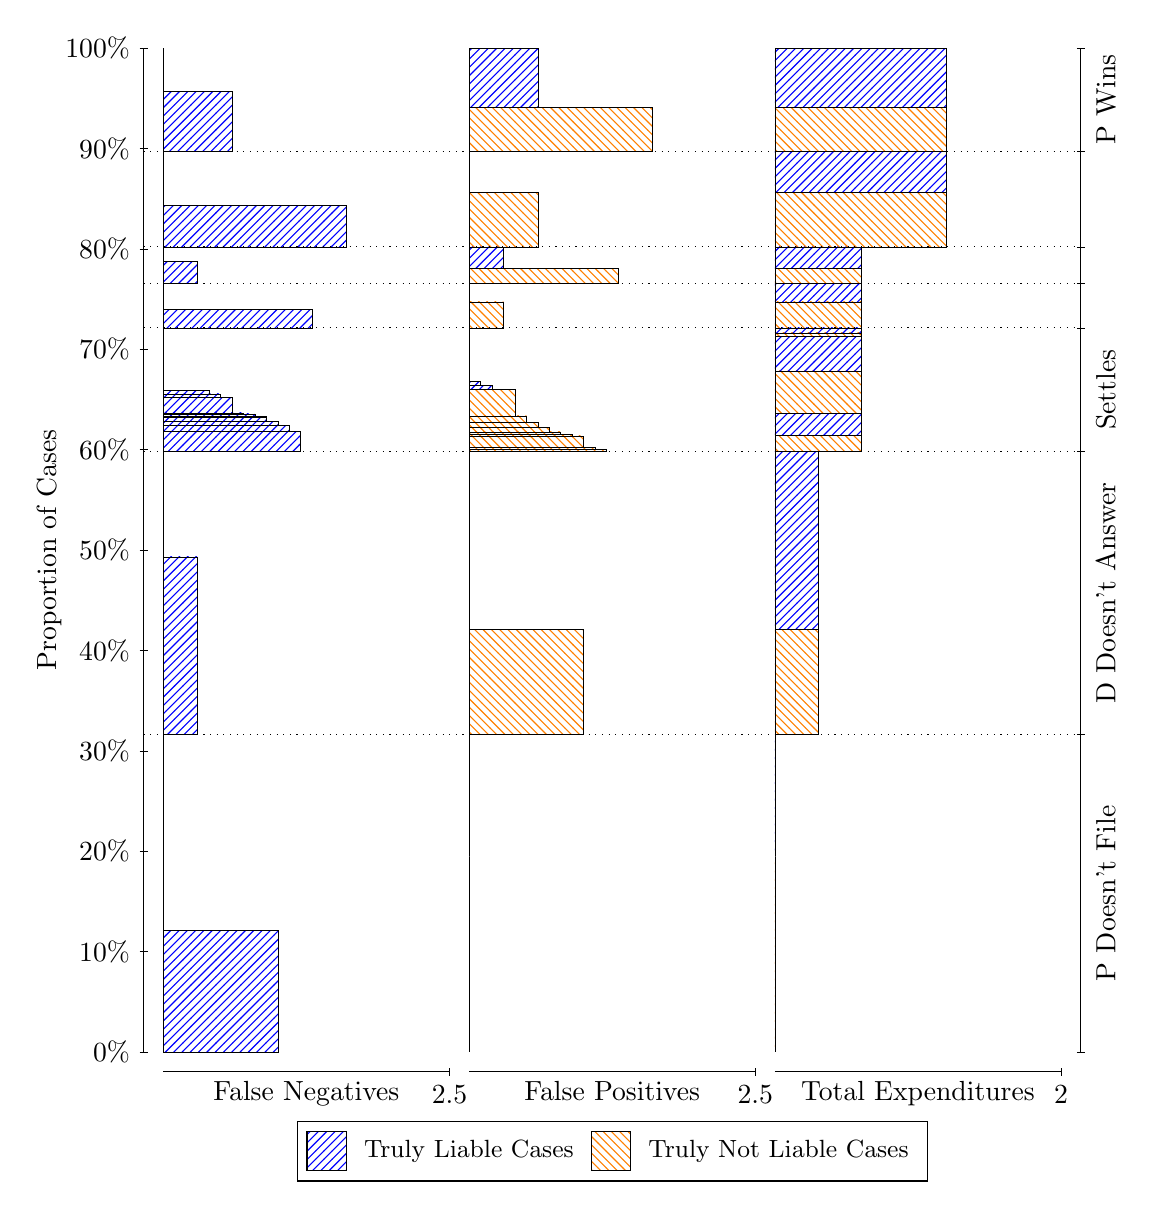
\begin{tikzpicture}
\draw[black, very thin] (1.5,1.75) -- (1.5,14.5);
\node[rotate=90, text=black, anchor=center] at (0.3, 8.125) {Proportion of Cases};
\draw[black, very thin] (1.45,1.75) -- (1.55,1.75);
\node[text=black, anchor=east] at (1.45, 1.75) {0\%};
\draw[black, very thin] (1.45,3.025) -- (1.55,3.025);
\node[text=black, anchor=east] at (1.45, 3.025) {10\%};
\draw[black, very thin] (1.45,4.3) -- (1.55,4.3);
\node[text=black, anchor=east] at (1.45, 4.3) {20\%};
\draw[black, very thin] (1.45,5.575) -- (1.55,5.575);
\node[text=black, anchor=east] at (1.45, 5.575) {30\%};
\draw[black, very thin] (1.45,6.85) -- (1.55,6.85);
\node[text=black, anchor=east] at (1.45, 6.85) {40\%};
\draw[black, very thin] (1.45,8.125) -- (1.55,8.125);
\node[text=black, anchor=east] at (1.45, 8.125) {50\%};
\draw[black, very thin] (1.45,9.4) -- (1.55,9.4);
\node[text=black, anchor=east] at (1.45, 9.4) {60\%};
\draw[black, very thin] (1.45,10.675) -- (1.55,10.675);
\node[text=black, anchor=east] at (1.45, 10.675) {70\%};
\draw[black, very thin] (1.45,11.95) -- (1.55,11.95);
\node[text=black, anchor=east] at (1.45, 11.95) {80\%};
\draw[black, very thin] (1.45,13.225) -- (1.55,13.225);
\node[text=black, anchor=east] at (1.45, 13.225) {90\%};
\draw[black, very thin] (1.45,14.5) -- (1.55,14.5);
\node[text=black, anchor=east] at (1.45, 14.5) {100\%};

\draw[black, very thin] (13.4,1.75) -- (13.4,14.5);
\draw[black, very thin] (13.35,1.75) -- (13.45,1.75);
\node[anchor=west] at (13.35, 1.75) {};
\draw[black, very thin] (13.35,5.7812) -- (13.45,5.7812);
\node[anchor=west] at (13.35, 5.7812) {};
\draw[black, very thin] (13.35,9.375) -- (13.45,9.375);
\node[anchor=west] at (13.35, 9.375) {};
\draw[black, very thin] (13.35,10.946) -- (13.45,10.946);
\node[anchor=west] at (13.35, 10.946) {};
\draw[black, very thin] (13.35,11.512) -- (13.45,11.512);
\node[anchor=west] at (13.35, 11.512) {};
\draw[black, very thin] (13.35,11.974) -- (13.45,11.974);
\node[anchor=west] at (13.35, 11.974) {};
\draw[black, very thin] (13.35,13.19) -- (13.45,13.19);
\node[anchor=west] at (13.35, 13.19) {};
\draw[black, very thin] (13.35,14.5) -- (13.45,14.5);
\node[anchor=west] at (13.35, 14.5) {};

\draw[black, very thin, pattern color=blue, pattern=north east lines] (1.75,1.75) rectangle (3.2033,3.2984);
\draw[black, very thin, pattern color=orange, pattern=north west lines] (1.75,3.2984) rectangle (1.75,5.7812);
\draw[black, very thin, pattern color=blue, pattern=north east lines] (1.75,5.7812) rectangle (2.186,8.037);
\draw[black, very thin, pattern color=orange, pattern=north west lines] (1.75,8.037) rectangle (1.75,9.375);
\draw[black, very thin, pattern color=blue, pattern=north east lines] (1.75,9.375) rectangle (3.494,9.6351);
\draw[black, very thin, pattern color=blue, pattern=north east lines] (1.75,9.6351) rectangle (3.3487,9.7085);
\draw[black, very thin, pattern color=blue, pattern=north east lines] (1.75,9.7085) rectangle (3.2033,9.7595);
\draw[black, very thin, pattern color=blue, pattern=north east lines] (1.75,9.7595) rectangle (3.058,9.8131);
\draw[black, very thin, pattern color=blue, pattern=north east lines] (1.75,9.8131) rectangle (3.058,9.8176);
\draw[black, very thin, pattern color=blue, pattern=north east lines] (1.75,9.8176) rectangle (2.9127,9.8547);
\draw[black, very thin, pattern color=blue, pattern=north east lines] (1.75,9.8547) rectangle (2.7673,9.8675);
\draw[black, very thin, pattern color=blue, pattern=north east lines] (1.75,9.8675) rectangle (2.622,10.059);
\draw[black, very thin, pattern color=blue, pattern=north east lines] (1.75,10.059) rectangle (2.4767,10.108);
\draw[black, very thin, pattern color=blue, pattern=north east lines] (1.75,10.108) rectangle (2.3313,10.155);
\draw[black, very thin, pattern color=orange, pattern=north west lines] (1.75,10.155) rectangle (1.75,10.946);
\draw[black, very thin, pattern color=blue, pattern=north east lines] (1.75,10.946) rectangle (3.6393,11.183);
\draw[black, very thin, pattern color=orange, pattern=north west lines] (1.75,11.183) rectangle (1.75,11.512);
\draw[black, very thin, pattern color=blue, pattern=north east lines] (1.75,11.512) rectangle (2.186,11.787);
\draw[black, very thin, pattern color=orange, pattern=north west lines] (1.75,11.787) rectangle (1.75,11.974);
\draw[black, very thin, pattern color=blue, pattern=north east lines] (1.75,11.974) rectangle (4.0753,12.497);
\draw[black, very thin, pattern color=orange, pattern=north west lines] (1.75,12.497) rectangle (1.75,13.19);
\draw[black, very thin, pattern color=blue, pattern=north east lines] (1.75,13.19) rectangle (2.622,13.946);
\draw[black, very thin, pattern color=orange, pattern=north west lines] (1.75,13.946) rectangle (1.75,14.5);
\draw[black, very thin, pattern color=orange, pattern=north west lines] (5.6333,1.75) rectangle (5.6333,4.2328);
\draw[black, very thin, pattern color=blue, pattern=north east lines] (5.6333,4.2328) rectangle (5.6333,5.7812);
\draw[black, very thin, pattern color=orange, pattern=north west lines] (5.6333,5.7812) rectangle (7.0867,7.1192);
\draw[black, very thin, pattern color=blue, pattern=north east lines] (5.6333,7.1192) rectangle (5.6333,9.375);
\draw[black, very thin, pattern color=orange, pattern=north west lines] (5.6333,9.375) rectangle (7.3773,9.4017);
\draw[black, very thin, pattern color=orange, pattern=north west lines] (5.6333,9.4017) rectangle (7.232,9.4323);
\draw[black, very thin, pattern color=orange, pattern=north west lines] (5.6333,9.4323) rectangle (7.0867,9.5754);
\draw[black, very thin, pattern color=orange, pattern=north west lines] (5.6333,9.5754) rectangle (6.9413,9.5884);
\draw[black, very thin, pattern color=orange, pattern=north west lines] (5.6333,9.5884) rectangle (6.796,9.6241);
\draw[black, very thin, pattern color=orange, pattern=north west lines] (5.6333,9.6241) rectangle (6.6507,9.6792);
\draw[black, very thin, pattern color=orange, pattern=north west lines] (5.6333,9.6792) rectangle (6.5053,9.7419);
\draw[black, very thin, pattern color=orange, pattern=north west lines] (5.6333,9.7419) rectangle (6.36,9.8295);
\draw[black, very thin, pattern color=orange, pattern=north west lines] (5.6333,9.8295) rectangle (6.2147,10.166);
\draw[black, very thin, pattern color=blue, pattern=north east lines] (5.6333,10.166) rectangle (5.924,10.213);
\draw[black, very thin, pattern color=blue, pattern=north east lines] (5.6333,10.213) rectangle (5.7787,10.263);
\draw[black, very thin, pattern color=blue, pattern=north east lines] (5.6333,10.263) rectangle (5.6333,10.946);
\draw[black, very thin, pattern color=orange, pattern=north west lines] (5.6333,10.946) rectangle (6.0693,11.275);
\draw[black, very thin, pattern color=blue, pattern=north east lines] (5.6333,11.275) rectangle (5.6333,11.512);
\draw[black, very thin, pattern color=orange, pattern=north west lines] (5.6333,11.512) rectangle (7.5227,11.699);
\draw[black, very thin, pattern color=blue, pattern=north east lines] (5.6333,11.699) rectangle (6.0693,11.974);
\draw[black, very thin, pattern color=orange, pattern=north west lines] (5.6333,11.974) rectangle (6.5053,12.667);
\draw[black, very thin, pattern color=blue, pattern=north east lines] (5.6333,12.667) rectangle (5.6333,13.19);
\draw[black, very thin, pattern color=orange, pattern=north west lines] (5.6333,13.19) rectangle (7.9587,13.744);
\draw[black, very thin, pattern color=blue, pattern=north east lines] (5.6333,13.744) rectangle (6.5053,14.5);
\draw[black, very thin, pattern color=orange, pattern=north west lines] (9.5167,1.75) rectangle (9.5167,4.2328);
\draw[black, very thin, pattern color=blue, pattern=north east lines] (9.5167,4.2328) rectangle (9.5167,5.7812);
\draw[black, very thin, pattern color=orange, pattern=north west lines] (9.5167,5.7812) rectangle (10.062,7.1192);
\draw[black, very thin, pattern color=blue, pattern=north east lines] (9.5167,7.1192) rectangle (10.062,9.375);
\draw[black, very thin, pattern color=orange, pattern=north west lines] (9.5167,9.375) rectangle (10.607,9.5845);
\draw[black, very thin, pattern color=blue, pattern=north east lines] (9.5167,9.5845) rectangle (10.607,9.8623);
\draw[black, very thin, pattern color=orange, pattern=north west lines] (9.5167,9.8623) rectangle (10.607,10.401);
\draw[black, very thin, pattern color=blue, pattern=north east lines] (9.5167,10.401) rectangle (10.607,10.839);
\draw[black, very thin, pattern color=orange, pattern=north west lines] (9.5167,10.839) rectangle (10.607,10.882);
\draw[black, very thin, pattern color=blue, pattern=north east lines] (9.5167,10.882) rectangle (10.607,10.946);
\draw[black, very thin, pattern color=orange, pattern=north west lines] (9.5167,10.946) rectangle (10.607,11.275);
\draw[black, very thin, pattern color=blue, pattern=north east lines] (9.5167,11.275) rectangle (10.607,11.512);
\draw[black, very thin, pattern color=orange, pattern=north west lines] (9.5167,11.512) rectangle (10.607,11.699);
\draw[black, very thin, pattern color=blue, pattern=north east lines] (9.5167,11.699) rectangle (10.607,11.974);
\draw[black, very thin, pattern color=orange, pattern=north west lines] (9.5167,11.974) rectangle (11.697,12.667);
\draw[black, very thin, pattern color=blue, pattern=north east lines] (9.5167,12.667) rectangle (11.697,13.19);
\draw[black, very thin, pattern color=orange, pattern=north west lines] (9.5167,13.19) rectangle (11.697,13.744);
\draw[black, very thin, pattern color=blue, pattern=north east lines] (9.5167,13.744) rectangle (11.697,14.5);
\draw[black, dotted] (1.5,5.7812) -- (13.4,5.7812);
\draw[black, dotted] (1.5,9.375) -- (13.4,9.375);
\draw[black, dotted] (1.5,10.946) -- (13.4,10.946);
\draw[black, dotted] (1.5,11.512) -- (13.4,11.512);
\draw[black, dotted] (1.5,11.974) -- (13.4,11.974);
\draw[black, dotted] (1.5,13.19) -- (13.4,13.19);
\draw[black, very thin] (1.75,1.5) -- (5.3833,1.5);
\node[text=black, anchor=north] at (3.5667, 1.5) {False Negatives};
\draw[black, very thin] (5.3833,1.45) -- (5.3833,1.55);
\node[text=black, anchor=north] at (5.3833, 1.45) {2.5};

\draw[black, very thin] (5.6333,1.5) -- (9.2667,1.5);
\node[text=black, anchor=north] at (7.45, 1.5) {False Positives};
\draw[black, very thin] (9.2667,1.45) -- (9.2667,1.55);
\node[text=black, anchor=north] at (9.2667, 1.45) {2.5};

\draw[black, very thin] (9.5167,1.5) -- (13.15,1.5);
\node[text=black, anchor=north] at (11.333, 1.5) {Total Expenditures};
\draw[black, very thin] (13.15,1.45) -- (13.15,1.55);
\node[text=black, anchor=north] at (13.15, 1.45) {2};

\node[text=black, centered, rotate=90] at (13.72, 3.7656) {P Doesn't File};
\node[text=black, centered, rotate=90] at (13.72, 7.5781) {D Doesn't Answer};
\node[text=black, centered, rotate=90] at (13.72, 10.161) {Settles};



\node[text=black, centered, rotate=90] at (13.72, 13.845) {P Wins};

\draw (7.449999999999999,1.5) node[draw=none] (baseCoordinate) {};
\begin{scope}[align=center]
        \matrix[scale=0.5, draw=black, below=0.5cm of baseCoordinate, nodes={draw}, column sep=0.1cm]{
            \node[rectangle, draw, minimum width=0.5cm, minimum height=0.5cm, pattern color=blue, pattern=north east lines] {}; &
            \node[draw=none, font=\small, text=black] (B) {Truly Liable Cases}; &
            \node[rectangle, draw, minimum width=0.5cm, minimum height=0.5cm, pattern color=orange, pattern=north west lines] {}; &
            \node[draw=none, font=\small, text=black] (B) {Truly Not Liable Cases}; \\
            };
\end{scope}

\end{tikzpicture}
\end{document}